% Assignment 3 report: IoT Sensor Ingestion Service, load balancing and observability.
% LaTeX version of REPORT.md. Compile with pdfLaTeX (Overleaf default). Figures are in figures/.
\documentclass[11pt,a4paper]{article}

\usepackage[T1]{fontenc}
\usepackage[utf8]{inputenc}
\usepackage{lmodern}
\usepackage[a4paper,margin=2.2cm]{geometry}
\usepackage{microtype}
\usepackage{graphicx}
\usepackage{booktabs}
\usepackage{tabularx}
\usepackage{array}
\usepackage[font=small,labelfont=bf]{caption}
\usepackage{subcaption}
\usepackage{xcolor}
\usepackage{listings}
\usepackage{enumitem}
\usepackage{amsmath}
\usepackage{placeins}
\usepackage[colorlinks=true,linkcolor=blue!50!black,urlcolor=blue!50!black]{hyperref}
\urlstyle{tt}

% Sections lettered like the brief: A, A.1, ...
\renewcommand{\thesection}{\Alph{section}}
\setlist{itemsep=2pt,topsep=3pt}
\newcolumntype{Y}{>{\raggedright\arraybackslash}X}
\setlength{\parskip}{4pt}
\setlength{\parindent}{0pt}

% Repository files are linked to GitHub.
\newcommand{\repo}{https://github.com/affan002/ESD_hw3/blob/main}
\newcommand{\file}[1]{\href{\repo/#1}{\path{#1}}}

\lstset{basicstyle=\ttfamily\scriptsize,breaklines=true,breakatwhitespace=false,
        columns=fullflexible,frame=single,framerule=0.3pt,rulecolor=\color{black!30},
        backgroundcolor=\color{black!3},xleftmargin=2pt,xrightmargin=2pt}

\title{\textbf{IoT Sensor Ingestion Service:\\Load Balancing and Observability}}
\author{Muhammad Affan\\[2pt]\small Enterprise Software Development, Fall 2026 --- Assignment 3 (individual submission)}
\date{November 2026}

\begin{document}
\maketitle

\begin{itemize}
  \item \textbf{Extends Assignment 2}, which is frozen at git tag \path{a2-submission} (its report is \path{REPORT.md} at that tag; Assignment 1 is at \path{a1-submission}). This report covers only what Assignment 3 adds.
  \item \textbf{Repository:} \url{https://github.com/affan002/ESD_hw3}. \textbf{Run, experiment and recover:} \file{README.md}. \textbf{Design decisions} A3-1 to A3-18 (choice, reason, rejected alternative): \file{docs/DECISIONS.md}. \textbf{Stage evidence} with commands and output: \file{docs/BUILD_LOG.md}, sections A3-1 to A3-9. \textbf{Raw results:} \href{https://github.com/affan002/ESD_hw3/tree/main/docs/results/a3}{\path{docs/results/a3/}}.
  \item \textbf{Run conditions:} one laptop (8 CPU threads, 7.7\,GB RAM), Docker Compose, Envoy v1.40.2 with 2 worker threads. Workload for every run: \textbf{50 requests/s for 120\,s, open loop, one interface at a time}, no client retries or circuit breaker, no Envoy retries. All times are UTC unless a caption says otherwise.
\end{itemize}

% =====================================================================
\section{Replicas and routing}

\subsection{Architecture}

\begin{figure}[htbp]
  \centering
  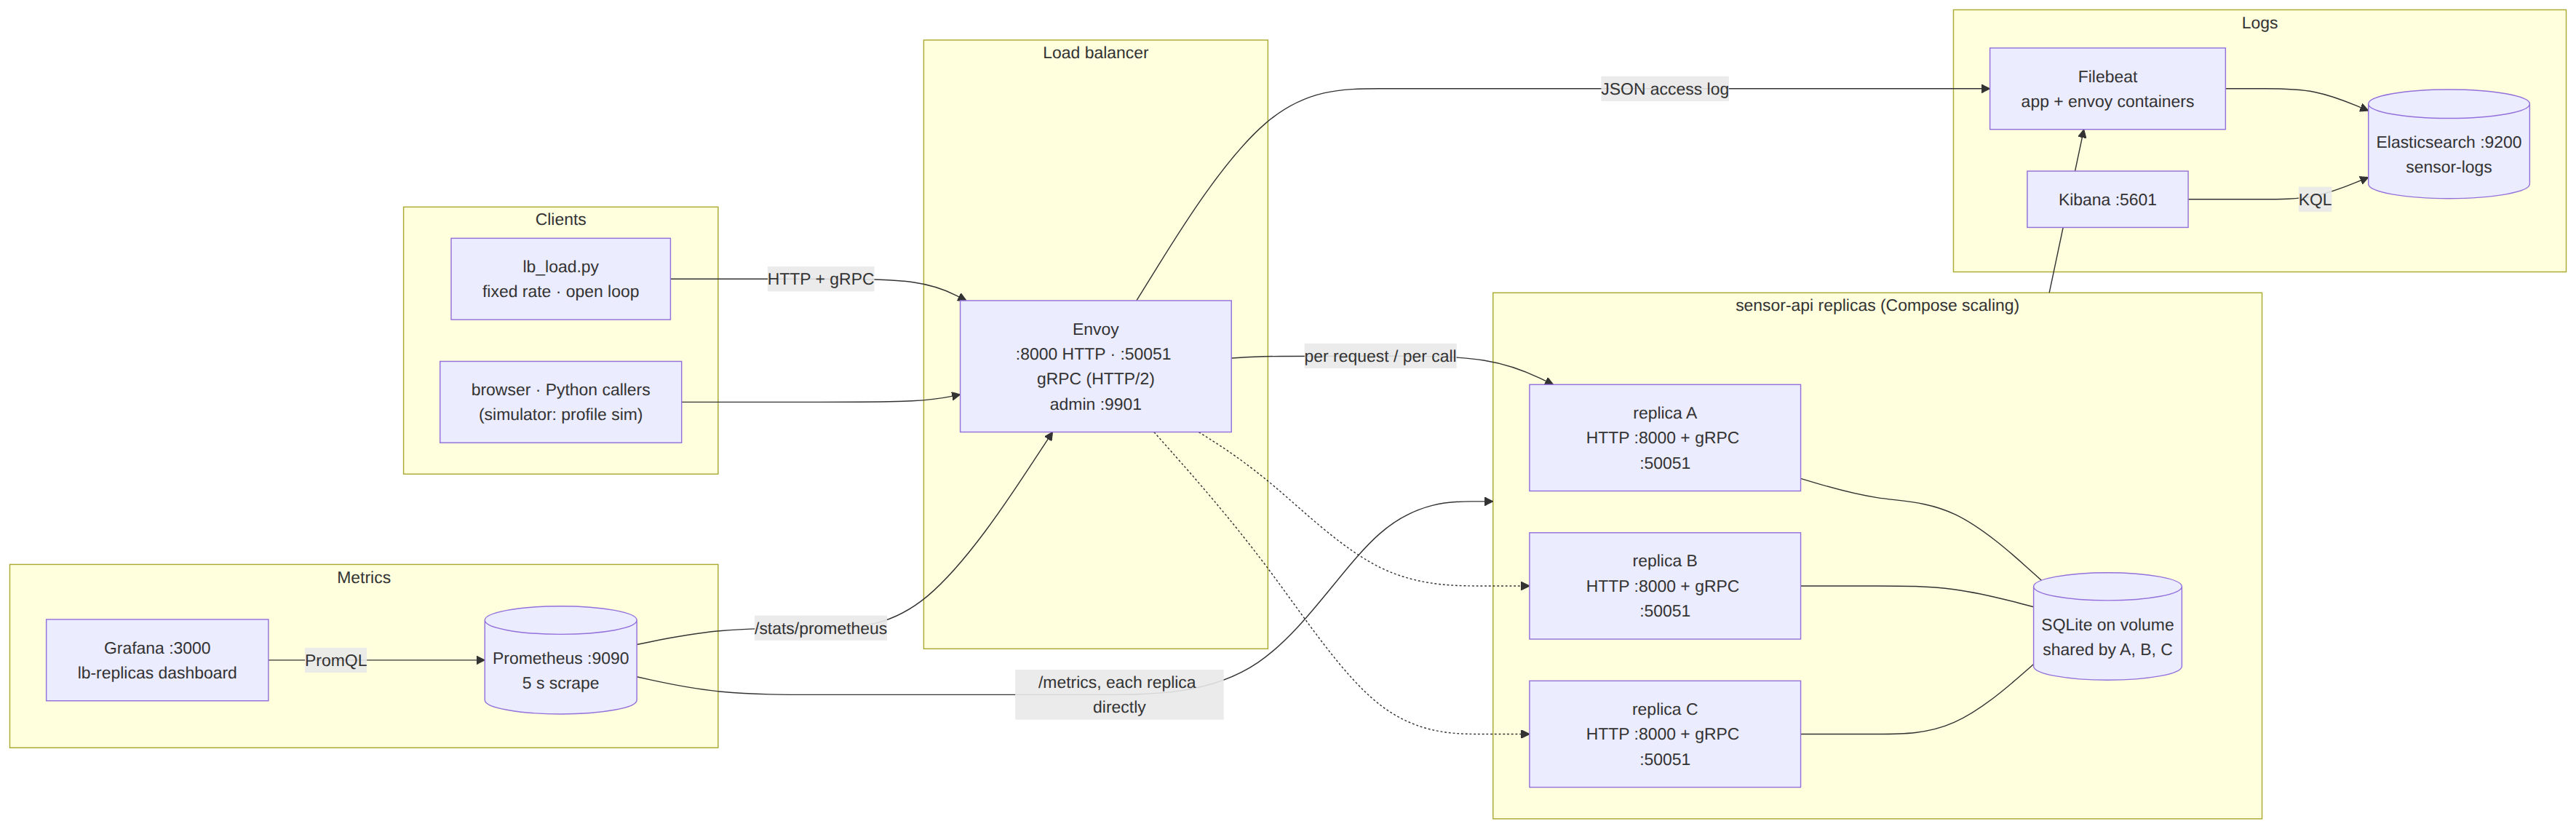
\includegraphics[width=\textwidth]{figures/architecture.png}
  \caption{Architecture. Clients reach Envoy only; Envoy forwards each HTTP request or gRPC call to replica A, B or C (dashed: destinations that depend on the active policy). The replicas share one SQLite file. Prometheus scrapes each replica and Envoy directly; Filebeat ships the replicas' logs and Envoy's access log to Elasticsearch.}
  \label{fig:arch}
\end{figure}

Replicas A, B and C are one Compose service scaled to 3 (\path{esd_hw3-app-1...3}). Each is \textbf{one process} serving HTTP (:8000) and gRPC (:50051), so both interfaces share one metrics registry and one fault switch (A3-2).

Envoy is the only entry point: HTTP on :8000 and gRPC on :50051 (HTTP/2), admin on :9901. Its clusters come from a watched file, so \path{scripts/lb_policy.sh <phase>} switches policy without a restart (A3-9). Prometheus scrapes each replica and Envoy directly; Filebeat ships both sets of JSON logs to Elasticsearch.

\subsection{Replica identity and correlation}

Scaled replicas share one environment, so each works out its name at start-up: a reverse-DNS lookup of its own IP returns \path{esd_hw3-app-2.esd_hw3_default}, and index 1/2/3 maps to A/B/C (A3-3). The name is on every log line (\path{replica}), in an \path{x-replica} response header or gRPC metadata, and in \path{sensor_replica_info}. It matches Prometheus's target label \path{replica} for all three. The \textbf{trace id is the request id}: the client's \path{x-request-id} is kept and logged by Envoy and by the replica (A3-5).

\subsection{Shared and per-replica state}

\begin{table}[htbp]
  \centering\small
  \caption{Where each kind of state lives.}
  \label{tab:state}
  \begin{tabularx}{\textwidth}{@{}p{2.6cm}p{3.6cm}p{1.7cm}Y@{}}
    \toprule
    State & Where & Shared? & Evidence \\
    \midrule
    Data (\path{readings}, \path{devices}) & One SQLite file on the \path{sensor-data} volume & \textbf{Shared} & The same \path{GET /devices/{id}} answer from every replica \\
    Idempotency records & Same table: unique index on \path{(device_id, recorded_at)} & \textbf{Shared} & One reading sent 3$\times$ through round robin: 201 from A (id 13), then 200 \emph{replayed} from B twice; the same key with a new value got 409 from C (\file{docs/results/a3/a_idempotency_cross_replica.txt}) \\
    Rate-limit buckets & Token bucket in each process's memory (\path{app/ratelimit.py}) & \textbf{Per replica} & A burst of 7 for one device: A only gives 5$\times$201 then 2$\times$429; round robin gives \textbf{7$\times$201} (\file{docs/results/a3/a_rate_limit_per_replica.txt}) \\
    \bottomrule
  \end{tabularx}
\end{table}

\textbf{What goes wrong with per-replica buckets:} behind round robin a device gets a burst of 5 \emph{per replica}, i.e.\ 15 at once and 3\,req/s, three times the configured limit, and the limit changes with the replica count. A shared store (SQLite, Redis) or consistent hashing on \path{device_id} would fix it; A3 keeps the buckets and documents the effect (A3-4).

\subsection{Test traffic}

HTTP \textbf{\path{GET /devices/{device_id}}} and gRPC \textbf{\path{GetDevice}} (a unary call added to the A2 service), with the same query and status rule. Being read-only, they avoid 429s and the SQLite write lock, so only the balancer differs between runs (A3-1).

\FloatBarrier
% =====================================================================
\section{Baseline: A only}

\subsection{Dashboard and queries}

Dashboard \textbf{``Load balancing $\cdot$ per replica''} (uid \path{lb-replicas}, exported at \file{monitoring/grafana/dashboards/lb-replicas.json}) has one row per interface plus an Envoy row. All panels use a \textbf{1-minute window}, which is at least 4$\times$ the 5\,s scrape interval.

\begin{table}[htbp]
  \centering\small
  \caption{Panel queries, per replica (HTTP shown; gRPC uses \texttt{sensor\_grpc\_*\{method="GetDevice"\}} and \texttt{code}).}
  \label{tab:promql}
  \begin{tabularx}{\textwidth}{@{}p{2.6cm}Y@{}}
    \toprule
    Panel & PromQL \\
    \midrule
    Request rate & \path{sum by (replica) (rate(sensor_http_requests_total{route="/devices/{device_id}"}[1m]))} \\
    Share of total & the same, \path{/ ignoring (replica) group_left sum(rate(...[1m]))}, with a dashed 1/3 reference line \\
    Active requests & \path{sum by (replica) (rate(sensor_http_request_duration_seconds_sum{...}[1m]))}: mean in flight by Little's law. The sampled \path{*_in_progress} gauge is shown dotted \\
    p50 / p95 & \path{histogram_quantile(q, sum by (replica, le) (rate(..._bucket{...}[1m])))} \\
    Errors by status & \path{sum by (replica, status_code) (rate(...{status_code!~"2.."}[1m])) > 0}, plus Envoy-only failures: \path{rate(envoy_cluster_upstream_rq_pending_failure_eject[1m])} + upstream timeouts \\
    Envoy & \path{envoy_cluster_endpoint_rq_total}, \path{envoy_cluster_membership_healthy}, health-check and connect failures \\
    \bottomrule
  \end{tabularx}
\end{table}

Labels are small fixed sets (\path{replica}, route/method, status, Envoy's endpoint hostname); request ids stay in logs. Active requests use Little's law because the sampled gauge rarely catches a 3\,ms call, and for HTTP it counts the \path{/metrics} scrape itself. Per-run numbers (\path{scripts/lb_run_stats.py}) sum raw samples over the run's range, since \path{increase()} extrapolates (1000 requests read as 1144, A3-15).

\subsection{Result}

\begin{table}[htbp]
  \centering\small
  \caption{Baseline, A only (50 req/s for 120\,s per interface).}
  \label{tab:baseline}
  \begin{tabular}{@{}lrrrrrc@{}}
    \toprule
    Interface & Rate & Sent & Successes & Failures & Client p95 & A / B / C \\
    \midrule
    HTTP & 50.01/s & 6000 & 6000 & 0 & 10.4\,ms & 6000 / 0 / 0 \\
    gRPC & 50.01/s & 6000 & 6000 & 0 & 9.5\,ms & 6000 / 0 / 0 \\
    \bottomrule
  \end{tabular}
\end{table}

\begin{figure}[htbp]
  \centering
  \begin{subfigure}{0.8\textwidth}\centering
    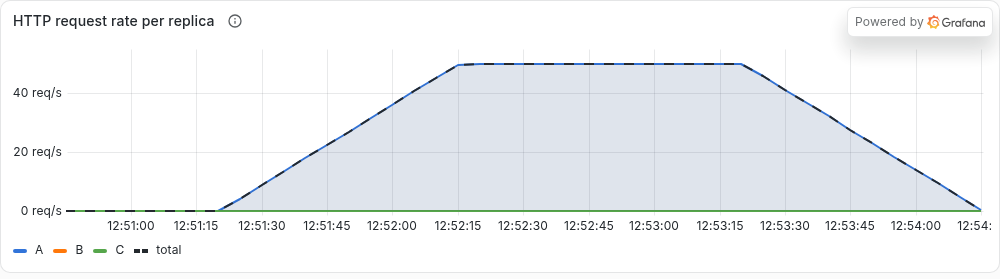
\includegraphics[width=\linewidth]{figures/b_baseline_http_rate.png}
    \caption{HTTP}
  \end{subfigure}\\[4pt]
  \begin{subfigure}{0.8\textwidth}\centering
    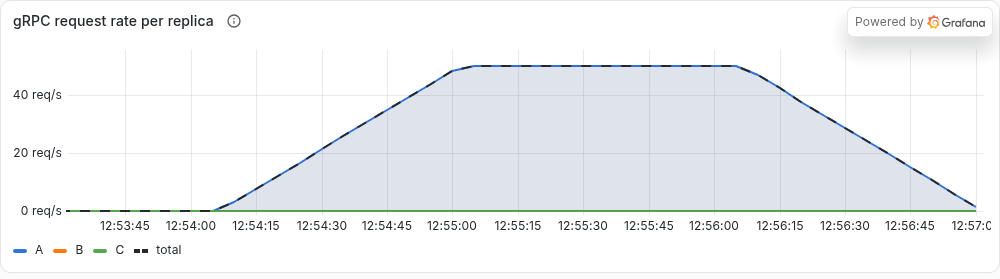
\includegraphics[width=\linewidth]{figures/b_baseline_grpc_rate.png}
    \caption{gRPC}
  \end{subfigure}
  \caption{Baseline request rate per replica. Only A has traffic: 50\,req/s (the ramps are the 1-minute window filling and emptying). B and C stay at 0 although they run and pass health checks.}
  \label{fig:baseline}
\end{figure}

A's server p95 was 9.7\,ms (HTTP) and 4.8\,ms (gRPC) with 0.27 and 0.12 requests in flight: one replica is far from busy at 50\,req/s. Client p95 adds 1--5\,ms for Envoy, the client and the network.

\subsection{Envoy event and replica event together}

One KQL query, \path{request_id : "<id>"}, returns Envoy's \path{envoy_access} event and the replica's own event (saved searches \path{sensor-envoy-http} / \path{sensor-envoy-grpc}).

\begin{figure}[htbp]
  \centering
  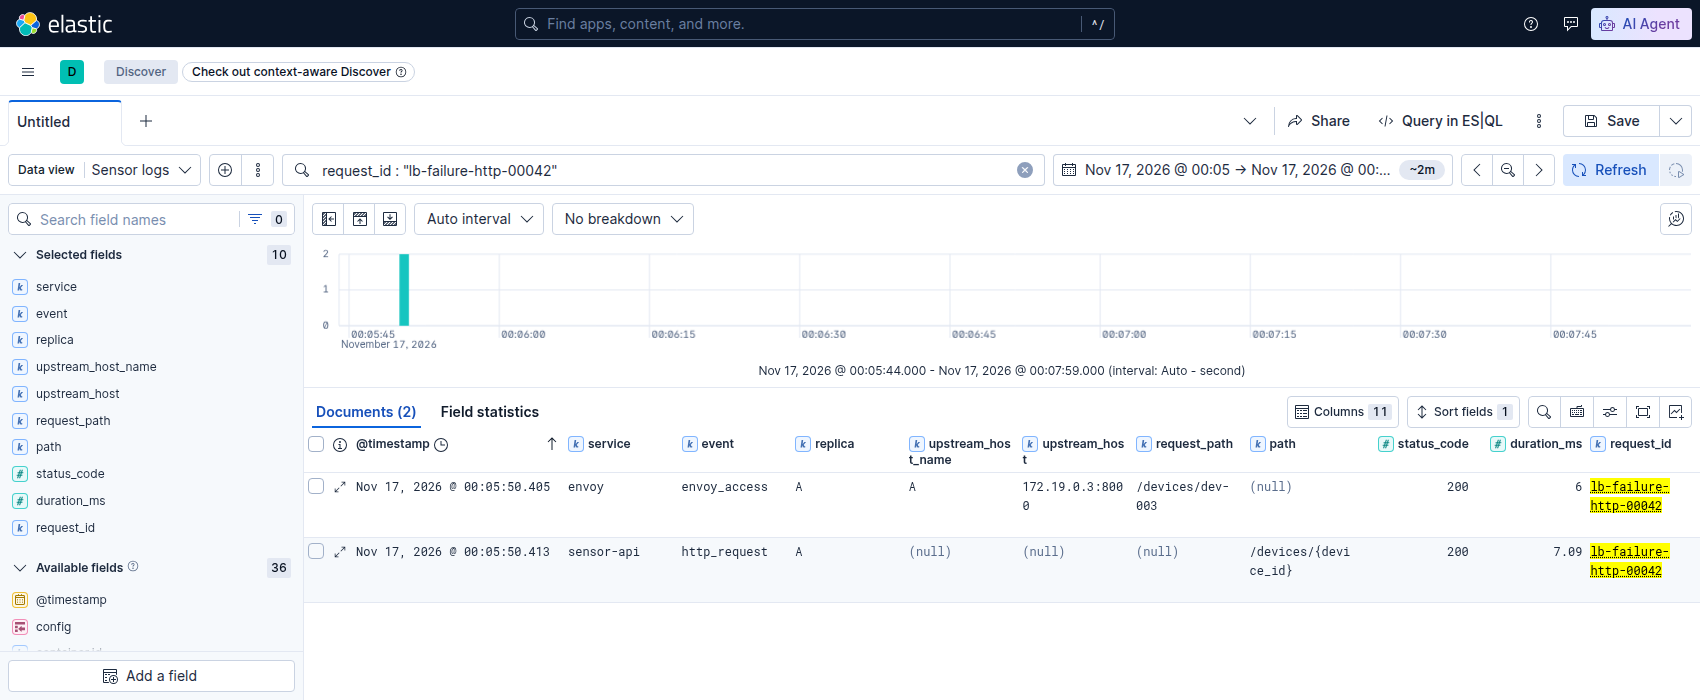
\includegraphics[width=\textwidth]{figures/b_kibana_http_envoy_and_replica.png}\\[4pt]
  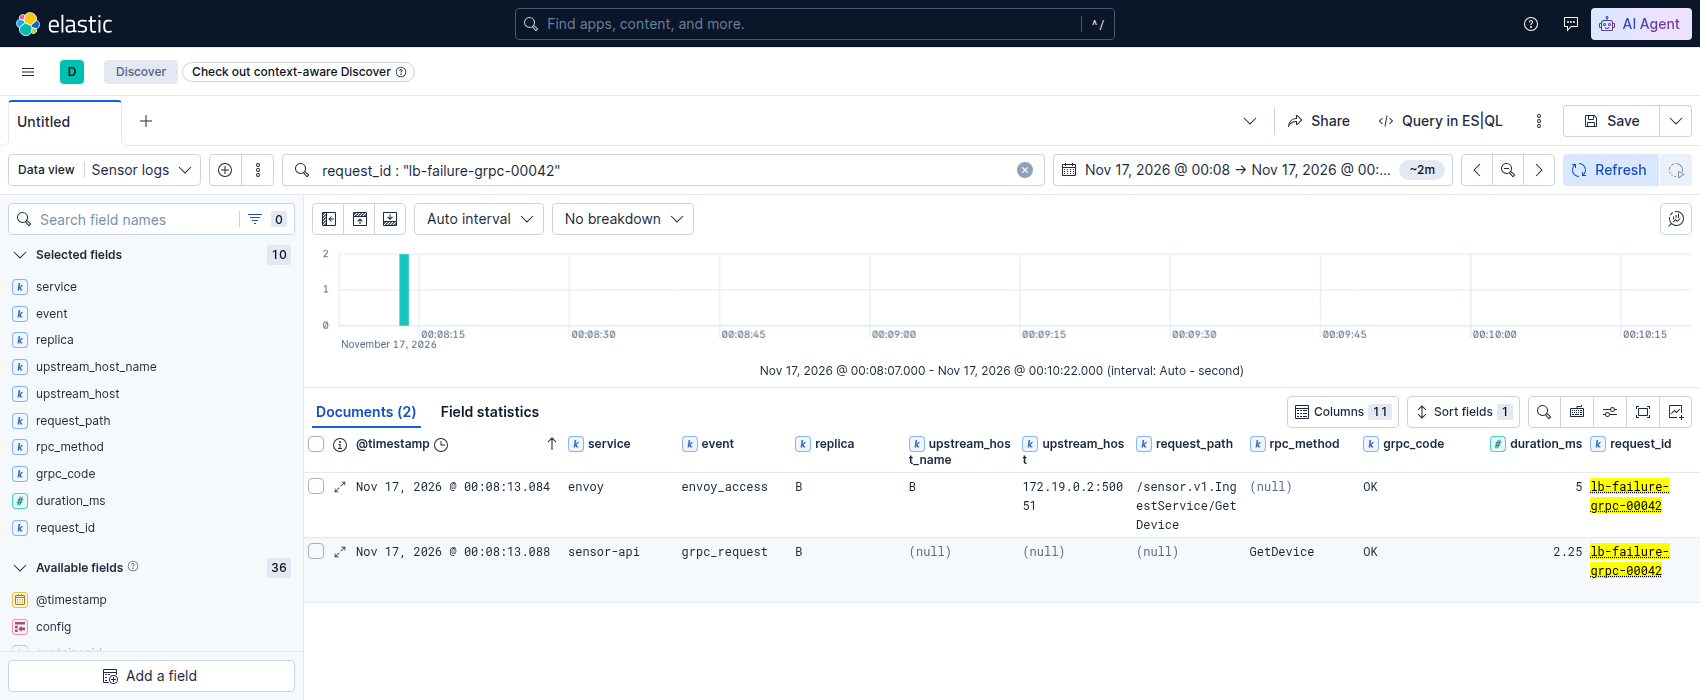
\includegraphics[width=\textwidth]{figures/b_kibana_grpc_envoy_and_replica.png}
  \caption{Kibana Discover, one search per interface (times in PKT, UTC+5). Top, HTTP: Envoy's line names the endpoint it picked (\texttt{upstream\_host\_name} A) and the replica that answered (\texttt{replica} A); A's own line follows 8\,ms later with its 7.09\,ms duration. Bottom, gRPC: the same for a \texttt{GetDevice} call that went to B, with \texttt{grpc\_code} OK on both lines.}
  \label{fig:kibana}
\end{figure}

The two proxy/backend log examples, as stored (\file{docs/results/a3/b_log_correlation.txt}, baseline run):

\begin{lstlisting}
{"service":"envoy","event":"envoy_access","replica":"A","upstream_host_name":"A","upstream_host":"172.19.0.3:8000","request_path":"/devices/dev-003","status_code":200,"duration_ms":6,"upstream_ms":"5","request_id":"lb-baseline-http-00042"}
{"service":"sensor-api","event":"http_request","replica":"A","path":"/devices/{device_id}","status_code":200,"duration_ms":6.28,"request_id":"lb-baseline-http-00042"}
{"service":"envoy","event":"envoy_access","replica":"A","upstream_host":"172.19.0.3:50051","request_path":"/sensor.v1.IngestService/GetDevice","status_code":200,"grpc_code":"OK","duration_ms":6,"request_id":"lb-baseline-grpc-00042"}
{"service":"sensor-api","event":"grpc_request","replica":"A","rpc_method":"GetDevice","grpc_code":"OK","duration_ms":2.84,"request_id":"lb-baseline-grpc-00042"}
\end{lstlisting}

\FloatBarrier
% =====================================================================
\section{Round robin}

\path{lb_policy.sh round-robin} adds B and C (weight 1) to both clusters.

\begin{table}[htbp]
  \centering\small
  \caption{Equal round robin.}
  \label{tab:rr}
  \begin{tabular}{@{}lcccc@{}}
    \toprule
    Interface & A / B / C requests & Shares & Client p95 & Server p95 (each) \\
    \midrule
    HTTP & 2001 / 2000 / 1999 & 33.4 / 33.3 / 33.3\,\% & 10.0\,ms & 9.7\,ms \\
    gRPC & 2000 / 2000 / 2000 & 33.3 / 33.3 / 33.3\,\% & 9.1\,ms & 4.8\,ms \\
    \bottomrule
  \end{tabular}
\end{table}

\begin{figure}[htbp]
  \centering
  \begin{subfigure}{0.8\textwidth}\centering
    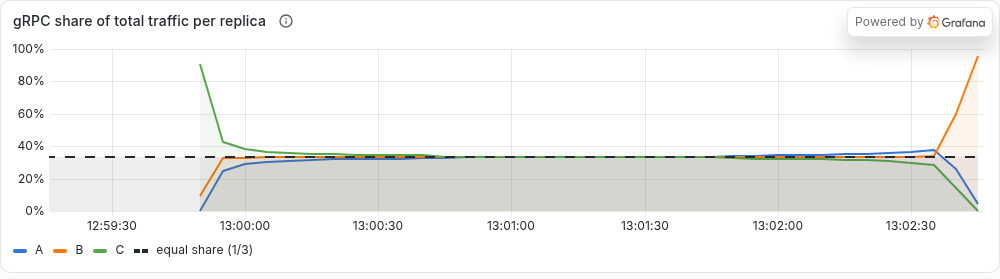
\includegraphics[width=\linewidth]{figures/c_round_robin_grpc_share.png}
    \caption{gRPC}
  \end{subfigure}\\[4pt]
  \begin{subfigure}{0.8\textwidth}\centering
    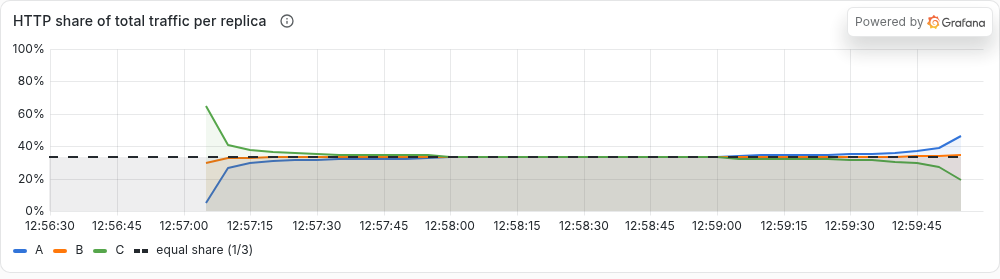
\includegraphics[width=\linewidth]{figures/c_round_robin_http_share.png}
    \caption{HTTP}
  \end{subfigure}
  \caption{Share of traffic per replica under round robin. All three shares sit on the dashed 1/3 reference line; the spikes at the edges are the ratio of near-zero rates while the 1-minute window fills and empties.}
  \label{fig:rr}
\end{figure}

\textbf{Versus 33\,\%:} gRPC's one connection sits on one Envoy worker, which cycles A$\rightarrow$B$\rightarrow$C exactly. HTTP opens a connection per request and Envoy's two workers keep separate round-robin positions, hence $\pm$1 (A3-16). \textbf{Versus the baseline:} latency is unchanged (same server p95, client p95 within 0.5\,ms), because one replica was not loaded; A's in-flight fell from 0.27 to 0.09. What changed is spare capacity, not speed.

\textbf{gRPC needs HTTP/2 routing:} through a \path{tcp_proxy} listener on the same cluster, each one-channel client run went 100\,\% to one replica (B, C, C); the HTTP/2 listener split it 334/333/333 (\file{docs/results/a3/c_grpc_tcp_vs_http2.txt}).

\FloatBarrier
% =====================================================================
\section{Experiments}

\subsection{Health checks and conditions}

\begin{table}[htbp]
  \centering\small
  \caption{Active health checks and proxy settings.}
  \label{tab:hc}
  \begin{tabularx}{\textwidth}{@{}YYY@{}}
    \toprule
    Setting & HTTP cluster & gRPC cluster \\
    \midrule
    Check & \path{GET /health} $\rightarrow$ 200 & \path{grpc.health.v1} \path{Check("")} $\rightarrow$ SERVING \\
    Interval / no-traffic interval & 2\,s / 2\,s & 2\,s / 2\,s \\
    Timeout & 1\,s & 1\,s \\
    Unhealthy / healthy threshold & 2 / 2 & 2 / 2 \\
    Connect timeout $\cdot$ DNS refresh & 1\,s $\cdot$ 5\,s & 1\,s $\cdot$ 5\,s \\
    Retries $\cdot$ outlier detection $\cdot$ circuit breakers & none $\cdot$ none $\cdot$ Envoy defaults (1024, never reached) & same \\
    \bottomrule
  \end{tabularx}
\end{table}

Each experiment started from round robin and was undone afterwards. Predictions were written before the runs and never edited (\file{docs/results/a3/d_predictions.md}).

\subsection{Weighted round robin 2:1:1}

\begin{itemize}
  \item \textbf{Prediction:} 50/25/25; no latency change; A has about 2$\times$ the requests in flight.
  \item \textbf{Observed:} HTTP 3001/1500/1499, gRPC 3000/1500/1500 (50/25/25\,\%). In flight: A 0.166 vs 0.084/0.083 (HTTP), 0.067 vs 0.034/0.035 (gRPC), i.e.\ 2$\times$. Server p95 unchanged; client p95 12.7 / 11.2\,ms.
  \item \textbf{Explanation:} a weight moves work, it doesn't add capacity. A at 25\,req/s is still mostly idle, so its service time is unchanged and its in-flight count doubles (Little's law). The 2\,ms client-p95 rise appears in no replica's p95, so it came from outside them (proxy, client or a memory-short host), not from the weights. Near saturation, double traffic would raise A's queueing, not its throughput.
\end{itemize}

\begin{figure}[htbp]
  \centering
  \begin{subfigure}{0.8\textwidth}\centering
    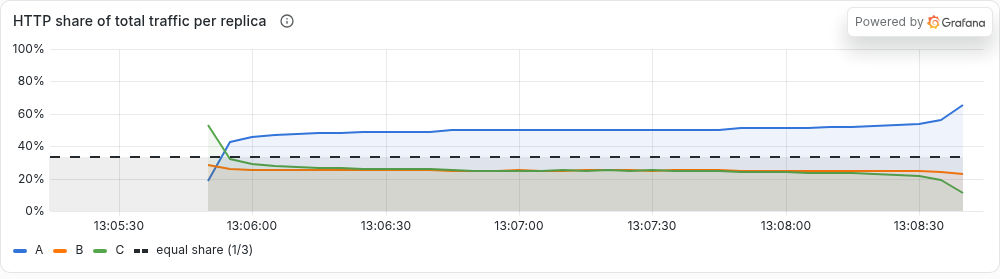
\includegraphics[width=\linewidth]{figures/d_weighted_http_share.png}
    \caption{Share of HTTP traffic}
  \end{subfigure}\\[4pt]
  \begin{subfigure}{0.8\textwidth}\centering
    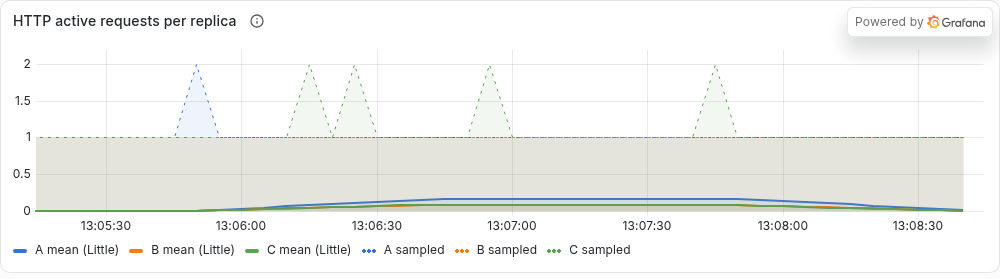
\includegraphics[width=\linewidth]{figures/d_weighted_http_active.png}
    \caption{HTTP active requests}
  \end{subfigure}
  \caption{Weighted round robin 2:1:1. (a) A holds 50\,\%, B and C overlap at 25\,\%. (b) A's mean in flight (solid, Little's law) is about twice B's and C's, all well below 1; the dotted gauge sits at 1 because it is read during Prometheus's own \texttt{/metrics} request, with occasional spikes to 2.}
  \label{fig:weighted}
\end{figure}

\subsection{Least request vs round robin, B delayed by 200\,ms}

B gets a 200\,ms delay on both interfaces; the same workload runs under round robin and under least request (Envoy's ``power of two choices'': pick 2 hosts at random, use the one with fewer active requests).

\begin{table}[htbp]
  \centering\small
  \caption{B delayed by 200\,ms: round robin (RR) vs least request (LR).}
  \label{tab:lr}
  \begin{tabular}{@{}llccc@{}}
    \toprule
    Run & Interface & A / B / C share & B in flight (mean) & Client p50 / p95 / mean \\
    \midrule
    Round robin & HTTP & 33.3 / 33.3 / 33.3\,\% & 3.45 & 10.9 / 212.0 / 76.8\,ms \\
    Round robin & gRPC & 33.3 / 33.3 / 33.3\,\% & 3.38 & 9.9 / 210.9 / 75.9\,ms \\
    Least request & HTTP & 43.0 / \textbf{13.8} / 43.3\,\% & \textbf{1.42} & 9.3 / 210.6 / \textbf{36.5}\,ms \\
    Least request & gRPC & 42.9 / \textbf{14.5} / 42.6\,\% & \textbf{1.47} & 9.1 / 210.1 / \textbf{37.8}\,ms \\
    \bottomrule
  \end{tabular}
\end{table}

\begin{figure}[htbp]
  \centering
  \begin{subfigure}{0.8\textwidth}\centering
    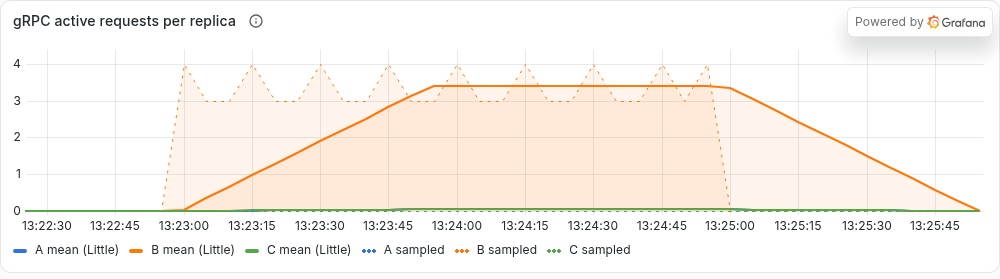
\includegraphics[width=\linewidth]{figures/d_delay_rr_grpc_active.png}
    \caption{Round robin}
  \end{subfigure}\\[4pt]
  \begin{subfigure}{0.8\textwidth}\centering
    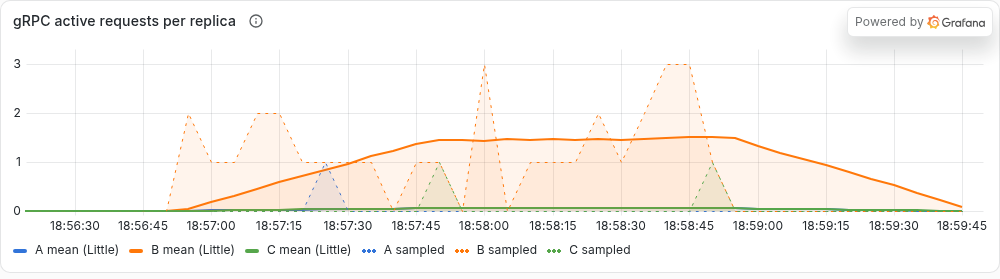
\includegraphics[width=\linewidth]{figures/d_delay_lr_grpc_active.png}
    \caption{Least request}
  \end{subfigure}
  \caption{gRPC active requests per replica with B delayed by 200\,ms. (a) Under round robin B's mean in flight climbs to about 3.4 and the sampled gauge reads 3--4. (b) Under least request it stays near 1.5, while A and C stay near 0.05 in both runs.}
  \label{fig:lr-active}
\end{figure}

\begin{figure}[htbp]
  \centering
  \begin{subfigure}{0.8\textwidth}\centering
    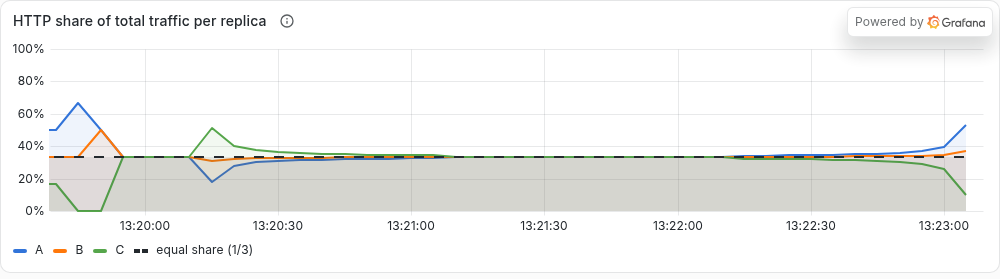
\includegraphics[width=\linewidth]{figures/d_delay_rr_http_share.png}
    \caption{Round robin}
  \end{subfigure}\\[4pt]
  \begin{subfigure}{0.8\textwidth}\centering
    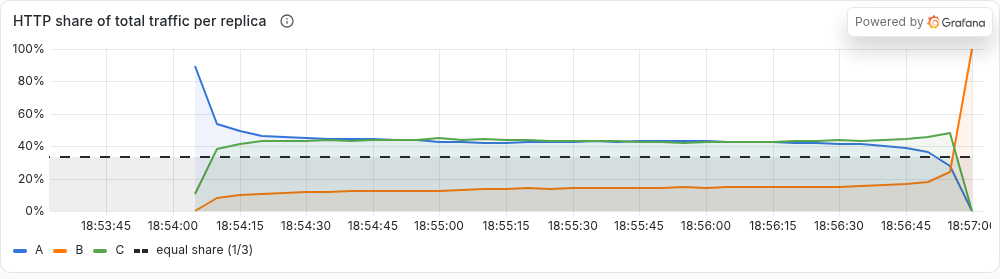
\includegraphics[width=\linewidth]{figures/d_delay_lr_http_share.png}
    \caption{Least request}
  \end{subfigure}
  \caption{Share of HTTP traffic with B delayed. (a) Round robin keeps all three on the 1/3 line, slow B included. (b) Least request moves traffic away from B: A and C settle near 43\,\% each and B near 14\,\%.}
  \label{fig:lr-share}
\end{figure}

\begin{itemize}
  \item \textbf{Prediction:} RR: B 33\,\%, $\approx$\,3.3 in flight, p95 $\approx$\,205\,ms. LR: B $\approx$\,10\,\%, $\approx$\,1 in flight, \textbf{p95 still $\approx$\,200\,ms}, mean lower.
  \item \textbf{Observed:} RR as predicted. LR: B 14\,\%, in flight 2.4$\times$ lower, mean halved, p95 unchanged.
  \item \textbf{Explanation:} RR ignores load, so B keeps a third and queues 16.7/s $\times$ 0.2\,s $\approx$ 3.4. LR avoids B whenever the other draw is less busy; B still wins when both draws are B (1/9) or on ties, so 14\,\% rather than 10\,\%. With 14\,\% $>$ 5\,\% of requests slow, the 95th percentile is still a slow one. \textbf{B passed every health check throughout}: health checks can't see a slow replica. (B's server p95 reads 242.5\,ms vs a true $\approx$\,205\,ms: interpolation inside the 100--250\,ms bucket.)
\end{itemize}

\subsection{Failure and recovery}

Round robin, no delay: \path{docker stop esd_hw3-app-2} at 30\,s, \path{docker start} at 70\,s; \path{scripts/lb_failure.py} polled Envoy's \path{/clusters} every 250\,ms.

\begin{table}[htbp]
  \centering\small
  \caption{Failure and recovery of replica B.}
  \label{tab:failure}
  \begin{tabular}{@{}lcc@{}}
    \toprule
     & HTTP & gRPC \\
    \midrule
    B removed (unhealthy) after \texttt{docker stop} issued & \textbf{3.6\,s} & \textbf{6.0\,s} \\
    Client errors & 54 $\times$ 503 (0.90\,\%) & 92 $\times$ \texttt{UNAVAILABLE} (1.53\,\%) \\
    B's own \texttt{/health} OK after \texttt{docker start} & 2.1\,s & 1.6\,s \\
    B healthy in Envoy after \texttt{docker start} & \textbf{4.8\,s} & \textbf{4.4\,s} \\
    A / B / C over the run & 39.4 / 21.2 / 39.4\,\% & 39.3 / 21.4 / 39.3\,\% \\
    \bottomrule
  \end{tabular}
\end{table}

Client timeline (HTTP): at $t$ = 29--32\,s about 17 of 50 requests/s failed (B's third), some after $\approx$\,0.9\,s; from $t$ = 33\,s A and C took 25/s each with no errors; B rejoined at $t$ = 74\,s, also without errors.

\begin{figure}[htbp]
  \centering
  \begin{subfigure}{0.8\textwidth}\centering
    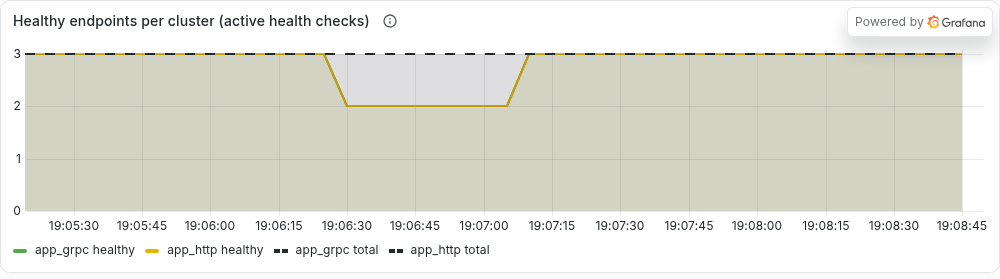
\includegraphics[width=\linewidth]{figures/d_failure_http_healthy.png}
    \caption{Healthy endpoints per cluster}
  \end{subfigure}\\[4pt]
  \begin{subfigure}{0.8\textwidth}\centering
    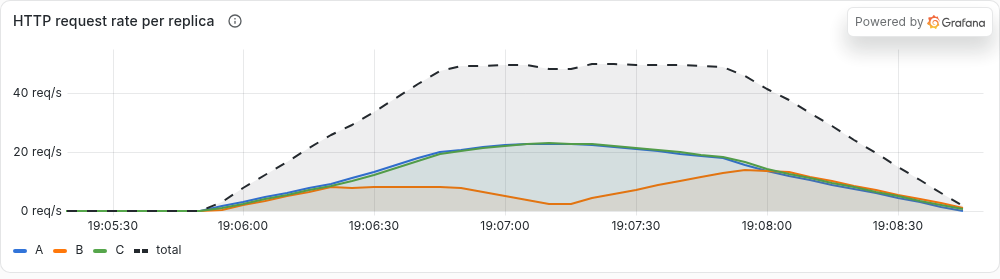
\includegraphics[width=\linewidth]{figures/d_failure_http_rate.png}
    \caption{HTTP request rate per replica}
  \end{subfigure}
  \caption{Failure run (HTTP). (a) Healthy endpoints drop from 3 to 2 after B's second failed check and return a few seconds after restart; both clusters move together because one container serves both interfaces. (b) B's rate dips while it is out and A and C rise to about 25\,req/s; the 1-minute window smooths the 4\,s gap into a broad dip, so the client's per-second timeline above is the precise view.}
  \label{fig:failure}
\end{figure}

\begin{figure}[htbp]
  \centering
  \begin{subfigure}{0.8\textwidth}\centering
    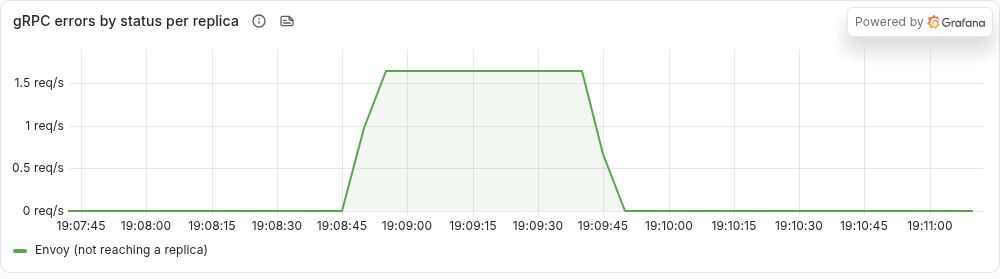
\includegraphics[width=\linewidth]{figures/d_failure_grpc_errors.png}
    \caption{gRPC}
  \end{subfigure}\\[4pt]
  \begin{subfigure}{0.8\textwidth}\centering
    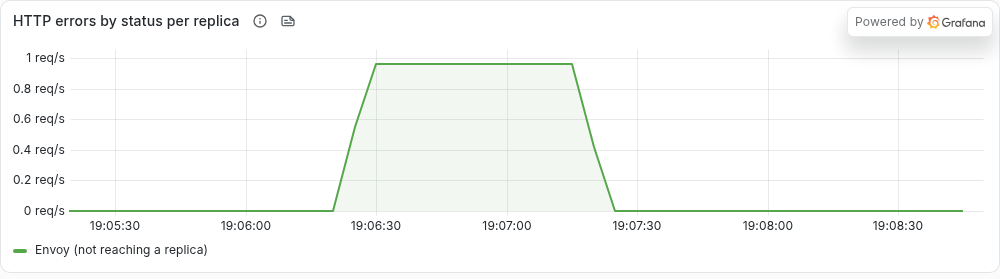
\includegraphics[width=\linewidth]{figures/d_failure_http_errors.png}
    \caption{HTTP}
  \end{subfigure}
  \caption{Errors during the failure runs. No replica saw an error: the failed calls never reached one. The only line is Envoy's \texttt{upstream\_rq\_pending\_failure\_eject} (requests failed because their upstream connection failed). (a) A 1-minute plateau at about 1.5/s, i.e.\ the 92 failures, returned as \texttt{UNAVAILABLE} inside HTTP 200, so an HTTP-5xx count would show nothing. (b) About 0.95/s, i.e.\ the 54 HTTP 503s.}
  \label{fig:failure-errors}
\end{figure}

\begin{figure}[htbp]
  \centering
  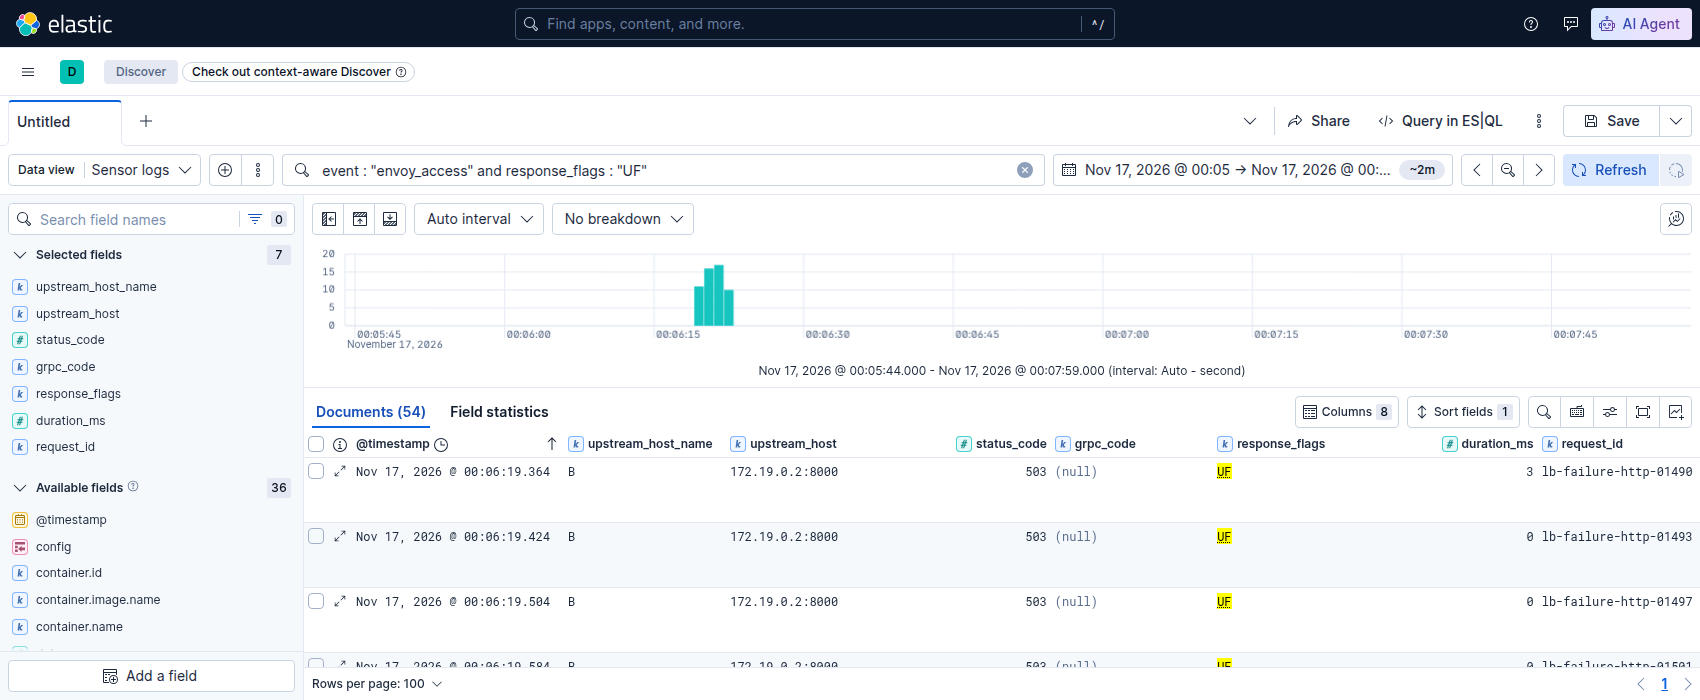
\includegraphics[width=\textwidth]{figures/d_kibana_failure_uf.png}
  \caption{Envoy access log in Kibana (times in PKT): \texttt{response\_flags : "UF"} finds the 54 HTTP 503s Envoy sent to B's address (\texttt{upstream\_host\_name} B); none of these request ids has a replica log line.}
  \label{fig:uf}
\end{figure}

\textbf{Timings vs settings.} Removal needs 2 failed checks. HTTP: B exited 1.1\,s after \texttt{stop} and the checks were refused at once, so it was out 2.5\,s later, consistent with two checks 2\,s apart. gRPC: with the container gone its IP stopped answering, so checks \textbf{timed out}; each failure then costs timeout + interval = 3\,s, and two take 4--6\,s (6.0\,s), which my 2--4\,s prediction missed. Until removal every request to B failed: errors $\approx \frac{1}{3} \times 50$/s $\times$ removal time (54, 92). Recovery = start-up (1.6--2.1\,s) + two passing checks $\approx$ 4.4--4.8\,s, within the predicted 4--7\,s, with no errors. A shorter interval, or one Envoy retry on connect failure (safe for read-only calls), would lose fewer requests.

\subsection{All runs}

From \file{docs/results/a3/summary.md}. Shares (of successes) equal Prometheus's and Envoy's per-endpoint counts in every run.

\begin{table}[htbp]
  \centering\footnotesize
  \caption{All runs (120\,s each, open loop, no retries).}
  \label{tab:summary}
  \begin{tabularx}{\textwidth}{@{}p{2.3cm}p{2.0cm}p{1.3cm}p{2.1cm}p{1.1cm}p{0.9cm}Y@{}}
    \toprule
    Run / interface & Policy and fault & Target / actual req/s & A / B / C (\%) & Client p95 & Errors & Explanation \\
    \midrule
    B baseline $\cdot$ HTTP & A only & 50 / 50.01 & 100 / 0 / 0 & 10.4\,ms & 0\,\% & Only A is a destination \\
    B baseline $\cdot$ gRPC & A only & 50 / 50.01 & 100 / 0 / 0 & 9.5\,ms & 0\,\% & same \\
    C round robin $\cdot$ HTTP & RR 1:1:1 & 50 / 50.01 & 33.4 / 33.3 / 33.3 & 10.0\,ms & 0\,\% & $\pm$1 from two workers' RR cycles \\
    C round robin $\cdot$ gRPC & RR 1:1:1 & 50 / 50.01 & 33.3 / 33.3 / 33.3 & 9.1\,ms & 0\,\% & Per-call routing over one connection \\
    D1 weighted $\cdot$ HTTP & RR 2:1:1 & 50 / 50.01 & 50.0 / 25.0 / 25.0 & 12.7\,ms & 0\,\% & A has 2$\times$ in flight; replicas not slower \\
    D1 weighted $\cdot$ gRPC & RR 2:1:1 & 50 / 50.01 & 50.0 / 25.0 / 25.0 & 11.2\,ms & 0\,\% & same \\
    D2 delay $\cdot$ RR $\cdot$ HTTP & RR, B +200\,ms & 50 / 50.01 & 33.3 / 33.3 / 33.3 & 212.0\,ms & 0\,\% & RR ignores B's queue (3.4 in flight) \\
    D2 delay $\cdot$ RR $\cdot$ gRPC & RR, B +200\,ms & 50 / 50.01 & 33.3 / 33.3 / 33.3 & 210.9\,ms & 0\,\% & same \\
    D2 delay $\cdot$ LR $\cdot$ HTTP & least request, B +200\,ms & 50 / 50.01 & 43.0 / 13.8 / 43.3 & 210.6\,ms & 0\,\% & B avoided; still $>$5\,\% slow, so p95 unchanged; mean halved \\
    D2 delay $\cdot$ LR $\cdot$ gRPC & least request, B +200\,ms & 50 / 50.01 & 42.9 / 14.5 / 42.6 & 210.1\,ms & 0\,\% & same \\
    D3 failure $\cdot$ HTTP & RR, B stopped 30--70\,s & 50 / 50.01 & 39.4 / 21.2 / 39.4 & 11.0\,ms & 0.90\,\% & Errors until 2 failed checks (3.6\,s) \\
    D3 failure $\cdot$ gRPC & RR, B stopped 30--70\,s & 50 / 50.01 & 39.3 / 21.4 / 39.3 & 10.1\,ms & 1.53\,\% & Timed-out checks: 6.0\,s to remove \\
    \bottomrule
  \end{tabularx}
\end{table}

\subsection{Cross-check with Envoy's access logs}

Weighted HTTP run (13:05:44--13:07:44): request ids \path{lb-weighted-http-*} grouped by Envoy's \path{upstream_host_name} give \textbf{A 3001 / B 1500 / C 1499}, equal to the client, Prometheus and the replicas' own events (\file{docs/results/a3/d_weighted_http_access_log.json}, \path{scripts/lb_es_check.py}). It holds for the failure run too (B: 1314 = 1260 OK + 54 \path{UF}). The check counts distinct ids, because a since-fixed Filebeat bug had re-shipped Envoy's log (24000 documents for 6000 requests, BUILD\_LOG A3-5).

\FloatBarrier
% =====================================================================
\section{Optional: consistent hashing and a fourth replica}

HTTP uses \path{RING_HASH} keyed on the path (\path{/devices/dev-NNN}), with each replica placed on the ring by its letter and given 1024 points. Then \path{docker compose up -d --scale app=4} adds D (A3-18; \path{scripts/lb_hash_demo.py}, 100 devices):

\begin{table}[htbp]
  \centering\small
  \caption{Devices per replica before and after adding D (ring hash, 1024 points per host).}
  \label{tab:hash}
  \begin{tabular}{@{}lccccl@{}}
    \toprule
     & A & B & C & D & Devices that changed replica \\
    \midrule
    3 replicas & 28 & 32 & 40 & -- & -- \\
    4 replicas & 20 & 27 & 31 & 22 & \textbf{22 / 100, all to D} (8 from A, 5 from B, 9 from C) \\
    D removed again & 28 & 32 & 40 & -- & 100 / 100 back on their original replica \\
    \bottomrule
  \end{tabular}
\end{table}

Every device got the same replica on repeated requests. The moved ids are listed in \file{docs/results/a3/e_consistent_hash.txt}, e.g.\ dev-002, dev-013, dev-014 $\rightarrow$ D. Naive \path{md5(id) % N} would have moved 72 of 100.

The first try used a fixed ring size (1024 points shared by all hosts). Adding D then took points away from A, B and C, so 40 devices moved, \textbf{12 of them between the old replicas} (\file{docs/results/a3/e_consistent_hash_shared_ring.txt}). The minimal-movement property needs a fixed number of points per host.

\FloatBarrier
% =====================================================================
\section*{Conclusions}
\addcontentsline{toc}{section}{Conclusions}

\begin{enumerate}
  \item \textbf{Least request for both interfaces, and for gRPC only on the HTTP/2 listener.} With healthy, identical replicas round robin was exact (33.3\,\%), so LR loses nothing; with one slow replica RR kept a third of traffic on it (3.4 queued, mean 77\,ms) while LR cut B to 14\,\%, its queue to 1.4 and the mean to 37\,ms on both interfaces. gRPC must be routed per call: \path{tcp_proxy} pinned a client 100\,\% to one replica. Neither policy fixed p95 ($\approx$\,210\,ms); that needs the slow host ejected (outlier detection), since health checks kept passing.
  \item \textbf{Differently:} if replicas keep per-device state in memory, like our rate-limit buckets, I'd use \textbf{consistent hashing on \path{device_id}} (ring hash or Maglev), so each device keeps one bucket; LR would spread a device over all replicas and triple its limit (Section~A.3).
  \item \textbf{If Envoy stops}, every call fails with connection refused although A, B and C are healthy, and Prometheus shows idle replicas, not errors: Envoy is a single point of failure. Improvement: two Envoys behind a floating virtual IP (keepalived/VRRP), or several proxy pods behind a Kubernetes Service, plus an alert on Envoy's \path{up} and on client errors.
\end{enumerate}

\section*{Credits and AI assistance}
\addcontentsline{toc}{section}{Credits and AI assistance}

\begin{itemize}
  \item Written with the help of Claude Code (Anthropic), which implemented the code and ran the experiments to my design decisions (\file{docs/DECISIONS.md}). I reviewed the code and checked the outputs recorded here.
  \item Reused: my own A1 and A2 code (tags \path{a1-submission}, \path{a2-submission}): the API, gRPC service, metrics, logging pipeline and the A1 load-script helpers.
  \item References: Envoy documentation on load balancing (round robin, weighted, least request, power of two choices), active health checking, the HTTP connection manager and \path{tcp_proxy}; Docker Compose documentation on service scaling; the gRPC health checking protocol (\path{grpc.health.v1}).
  \item Libraries and tools: FastAPI, Uvicorn, Pydantic, grpcio / grpcio-health-checking / protobuf, prometheus\_client, pytest, Envoy, Prometheus, Grafana, Filebeat, Elasticsearch, Kibana.
\end{itemize}

\end{document}
